
\chapter{DDOS Attacks}


\section{The threat from Denial of service (DoS) attacks}









\section{Overview of Software Defined Networking}

\acrfull{sdn} is a computer network, realised in software, characterised by the separation of the management plane from the data plane, as opposed to the traditional  network devices. Traditional network devices are proprietary and hardware based. The vendors are competing for customers, and integration of network devices from different vendors for the purpose of centralised management and control is not actively supported by the vendors.


The \acrfull{sdn} is managed by a software-based centralised \acrshort{sdn} Controller, controlling each \acrshort{sdn}-enabled network device via its Southbound interface. The network thus has a centralised management interface, as opposed to traditional networks devices, each controlled by a local network operating system.\footnote{Like Junos OS from Juniper, or Cisco IOS from Cisco} The \acrshort{sdn} controller controls the data flow of the entire network, by communicating with the data layer utilising open communication protocols.


\subsection{Software Defined Networking}
A number of papers, like \cite{rehmani2019software}\footnote{As well as several of the papers referenced by the authors of \cite{rehmani2019software}} suggests utilising \acrfull{sdn} for the management and monitoring of the \acrshort{sg} due to the flexibility of open standards, and the separate control plane, as described by  \cite{rehmani2019software}. Therefore, an introduction to \acrshort{sdn} is included, following the introduction to virtualisation of networking. 



\subsubsection{Virtualisation of Networking}

The continued development of increasingly powerful Personal Computers, was followed by the virtualisation of 
computing resources, enabling virtual computers running on virtualisation hosts. As a consequence, virtual networking, providing network connections between virtual machines, emerged. Following the single computer hosting a few virtual machines, was the physical data center, hosting a virtual data center featuring a large number of virtual machines hosted by several physical hosts sharing common networks and storage, communicating via virtual enterprise-grade networks. Following the the development of virtual networks, initially implementing virtualisation of conventional network connections, a new networking paradigm was invented: \acrfull{sdn}. 

 \begin{figure}[ht]
\centering
    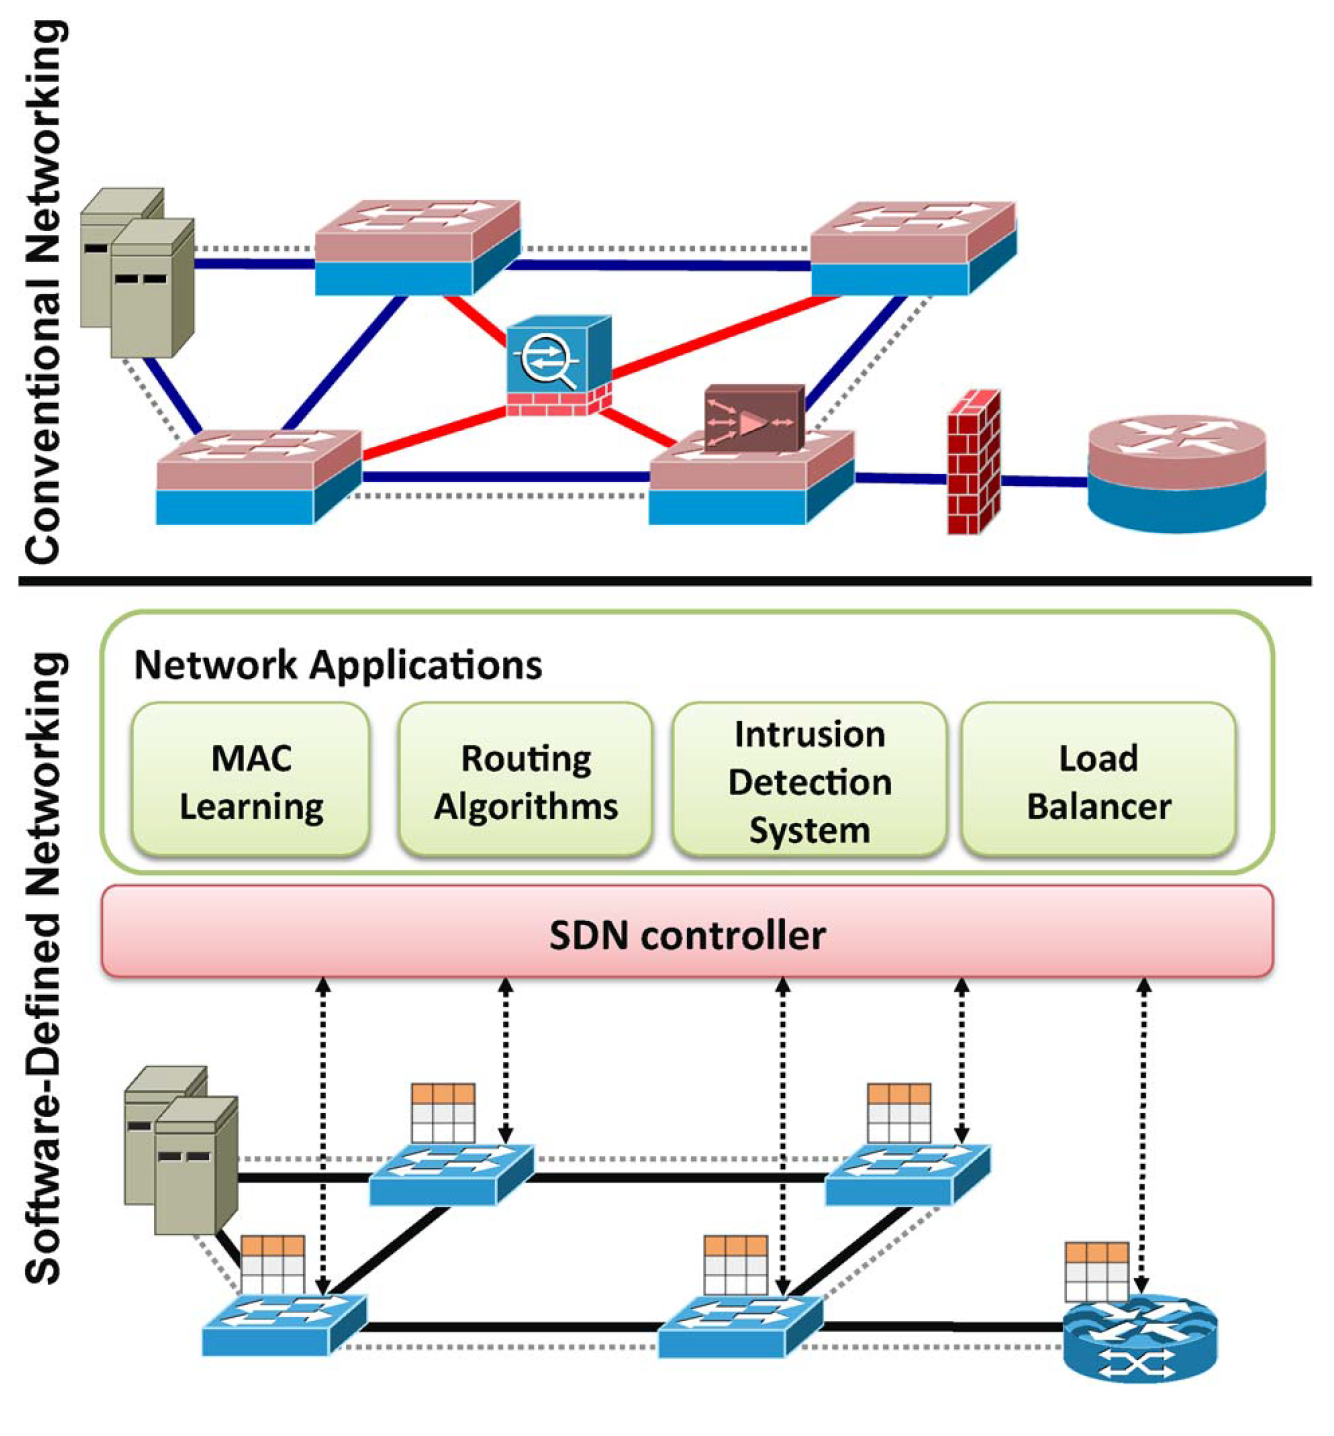
\includegraphics[width=\textwidth]{figures/SDNvsTradNetwork.png}
\caption{SDN vs Traditional Networking, as presented in \cite[p. 19]{kreutz2014software}}

\end{figure}



\section{The main components of the smart grid}
 The main components of smart grids such as
\begin{itemize}
\item smart sensors
\item Wired sensor networks, 
\item wireless sensor networks (WSNs).
\item phasor measurement unit (PMU), 
\item smart meters (SMs), 

\end{itemize}

smart grid applications and main requirements are
explained on the basis of advanced metering infrastructure (AMI), demand response
(DR), station and substation automation, and demand-side management (DSM).\\ 




A survey of the security of\acrlong{sdn}\cite{ALSMADI201579}:\\
\fullcite{ALSMADI201579}\\


Denial of service attacks utilises network connectivity and bandwidth limitations in order to obstruct service availability\cite{Asri_Pranggono_2015}. \\
 \fullcite{Asri_Pranggono_2015}\\ 

\begin{itemize}

\item{Examples of combining SDN and NFV to counter DDoS} 

\item{Utilising AI to detect DDoS} 

\item...
 

\item...


\item ...
\end{itemize}





\subsection{Case studies}
Several case studies exists related to \acrlong{sg}s countering DoS attacks.

 


\begin{itemize}
    \item Example 1  
    \begin{itemize}
        \item Description 
            \fullcite{demir2017towards}
        \item Security Assessment
        \item Summary
    \end{itemize}



\item Example 2
    \begin{itemize}
        \item Description 
           \fullcite{hameed2018sdn}
        \item Security Assessment
        \item Summary
    \end{itemize}


    \item Example 3  
    \begin{itemize}
        \item Description 
           \fullcite{jararweh2015software}
        \item Security Assessment
        \item Summary
    \end{itemize}
    
\end{itemize}




\subsection{Smart Grid DoS attack detection}
\subsection{Smart Grid DoS attack mitigation}
DDoS mitigation survey \fullcite{hameed2018sdn}



%sec 3


\subsection{The Demand For An Autonomous Control Mechanism}
As described in \cite{rehmani2019software}, the utilisation of \acrfull{sdn} is suggested in, order to meet the demands of automated control in Smart Grids.
\subsubsection{Advantages of utilising SDN}
\subsubsection{Vulnerabilities introduced by utilising SDN}



Therefore, the sucessful detection and mitigation of \acrlong{dos} attacks targeted against \acrlong{sg} also is important.\\ 

